\begin{figure}[htbp]
\centering
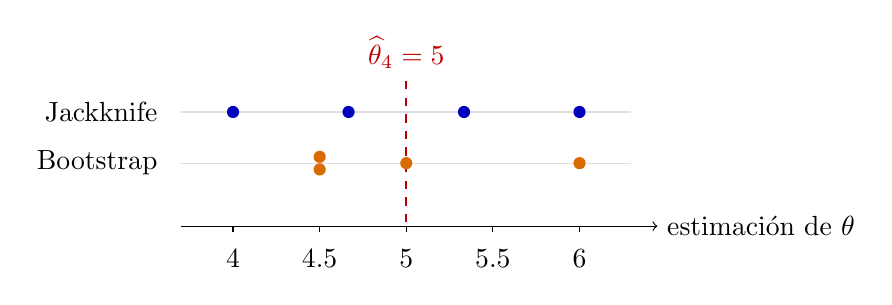
\begin{tikzpicture}[x=2.2cm,y=1cm]
  \draw[gray!25] (3.7,1.45) -- (6.3,1.45);
  \draw[gray!25] (3.7,0.8) -- (6.3,0.8);
  \draw[->] (3.7,0) -- (6.45,0)
    node[right] {estimación de $\theta$};
  \foreach \x/\lab in {4/4,4.5/4.5,5/5,5.5/5.5,6/6} {
    \draw (\x,0) -- (\x,-0.07) node[below=3pt] {$\lab$};
  }
  \node[anchor=east] at (3.62,1.45) {Jackknife};
  \node[anchor=east] at (3.62,0.8) {Bootstrap};
  \draw[dashed,red!75!black,thick] (5,0.05) -- (5,1.88);
  \node[above,red!75!black] at (5,1.88) {$\widehat\theta_4=5$};

  \foreach \x in {4,4.6667,5.3333,6}
    \fill[blue!75!black] (\x,1.45) circle (2.2pt);

  \fill[orange!85!black] (4.5,0.72) circle (2.2pt);
  \fill[orange!85!black] (4.5,0.88) circle (2.2pt);
  \fill[orange!85!black] (5,0.8) circle (2.2pt);
  \fill[orange!85!black] (6,0.8) circle (2.2pt);
\end{tikzpicture}
\caption{Estimaciones de eliminación jackknife y medias de las cuatro réplicas bootstrap del ejercicio. Los dos puntos apilados en $4.5$ corresponden a dos réplicas con la misma media; la línea roja señala la media de la muestra completa.}
\label{fig:integrador-clase3}
\end{figure}